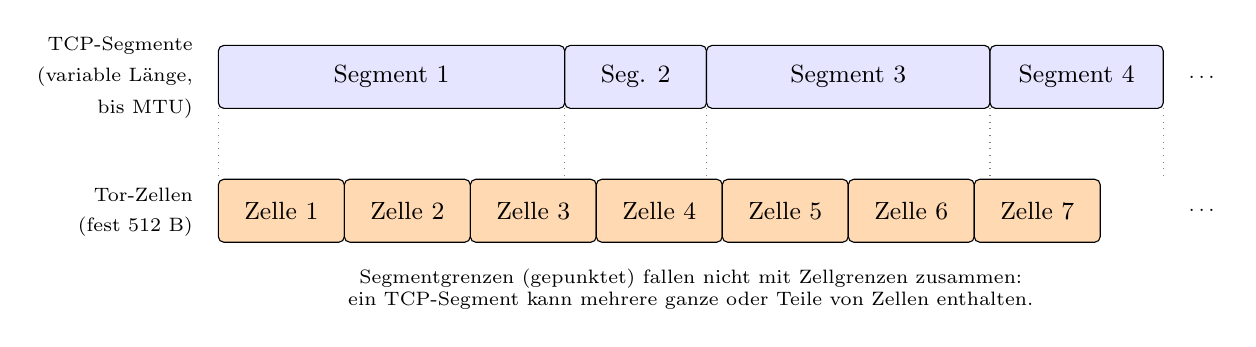
\begin{tikzpicture}[
    >=latex,
    every node/.style={font=\small},
    seg/.style={
        draw, rounded corners=2pt,
        minimum height=8mm,
        align=center, fill=blue!10
    },
    cell/.style={
        draw, rounded corners=2pt,
        minimum width=16mm, minimum height=8mm,
        align=center, fill=orange!30
    },
    lbl/.style={font=\scriptsize, anchor=east}
]

% ----------------------------------------------------------
% Obere Zeile: TCP-Segmente mit variabler Nutzdatengrösse
% ----------------------------------------------------------
\node[lbl] at (-2mm, 8mm) {TCP-Segmente};
\node[lbl] at (-2mm, 4mm) {(variable Länge,};
\node[lbl] at (-2mm, 0mm) {bis MTU)};

% Vier Segmente mit unterschiedlichen Breiten
\node[seg, minimum width=44mm] (s1) at (22mm, 4mm) {Segment 1};
\node[seg, minimum width=18mm] (s2) at (53mm, 4mm) {Seg. 2};
\node[seg, minimum width=36mm] (s3) at (80mm, 4mm) {Segment 3};
\node[seg, minimum width=22mm] (s4) at (109mm, 4mm) {Segment 4};

% ----------------------------------------------------------
% Mittlere Beschriftung
% ----------------------------------------------------------
\node[font=\scriptsize, anchor=west] at (122mm, 4mm) {\dots};

% ----------------------------------------------------------
% Untere Zeile: Tor-Zellen mit fester Grösse 512 B
% ----------------------------------------------------------
\node[lbl] at (-2mm, -11mm) {Tor-Zellen};
\node[lbl] at (-2mm, -15mm) {(fest 512 B)};

% Sieben Zellen, alle gleich breit, identisch hoch
\foreach \i [count=\j from 0] in {1,2,3,4,5,6,7} {
    \node[cell] at ({0mm + \j*16mm + 8mm}, -13mm) {Zelle \i};
}
\node[font=\scriptsize, anchor=west] at (122mm, -13mm) {\dots};

% ----------------------------------------------------------
% Verbindungslinien zwischen den Ebenen (Encapsulation)
% Sie zeigen, dass Segment- und Zellgrenzen nicht zusammenfallen
% ----------------------------------------------------------
\draw[dotted, gray] (0mm, 0mm)    -- (0mm, -9mm);
\draw[dotted, gray] (44mm, 0mm)   -- (44mm, -9mm);
\draw[dotted, gray] (62mm, 0mm)   -- (62mm, -9mm);
\draw[dotted, gray] (98mm, 0mm)   -- (98mm, -9mm);
\draw[dotted, gray] (120mm, 0mm)  -- (120mm, -9mm);

% ----------------------------------------------------------
% Erklärender Hinweis
% ----------------------------------------------------------
\node[font=\scriptsize, align=center] at (60mm, -23mm)
    {Segmentgrenzen (gepunktet) fallen nicht mit Zellgrenzen zusammen:\\
     ein TCP-Segment kann mehrere ganze oder Teile von Zellen enthalten.};

\end{tikzpicture}
